\section{Filtros Pasaaltos}
Se simularon los siguientes filtros pasaaltos con sus respectivas ventanas en MATLAB.

\begin{table}[H]
\centering
\begin{tabular}{|c|c|c|c|c|c|}
\hline
$f_s(Hz)$ & $f_p(Hz)$ & $f_a(Hz)$ & $A_p(dB)$ & $A_a(dB)$ & Ventana     \\ \hline
$44.1k$   & $1k$      & $2k$      & 2         & 20        & Rectangular \\
$44.1k$   & $1k$      & $2k$      & 2         & 40        & Hamming     \\
$44.1k$   & $1k$      & $2k$      & 1         & 40        & Blackman    \\
$44.1k$   & $2.4k$    & $3.6k$    & 2         & 40        & Kaiser      \\
$44.1k$   & $1k$      & $2k$      & 2         & 60        & Kaiser      \\ \hline
\end{tabular}
\caption{Plantillas de filtros pasaaltos realizados.}
\label{tab:plantillaspasaaltos}
\end{table}

\subsection{Ventana Rectangular}
La ventana rectangular está definida por:
\begin{equation}
    \omega (n+1)=1 \qquad  0<n<N-1
\end{equation}
\begin{figure}[H]
  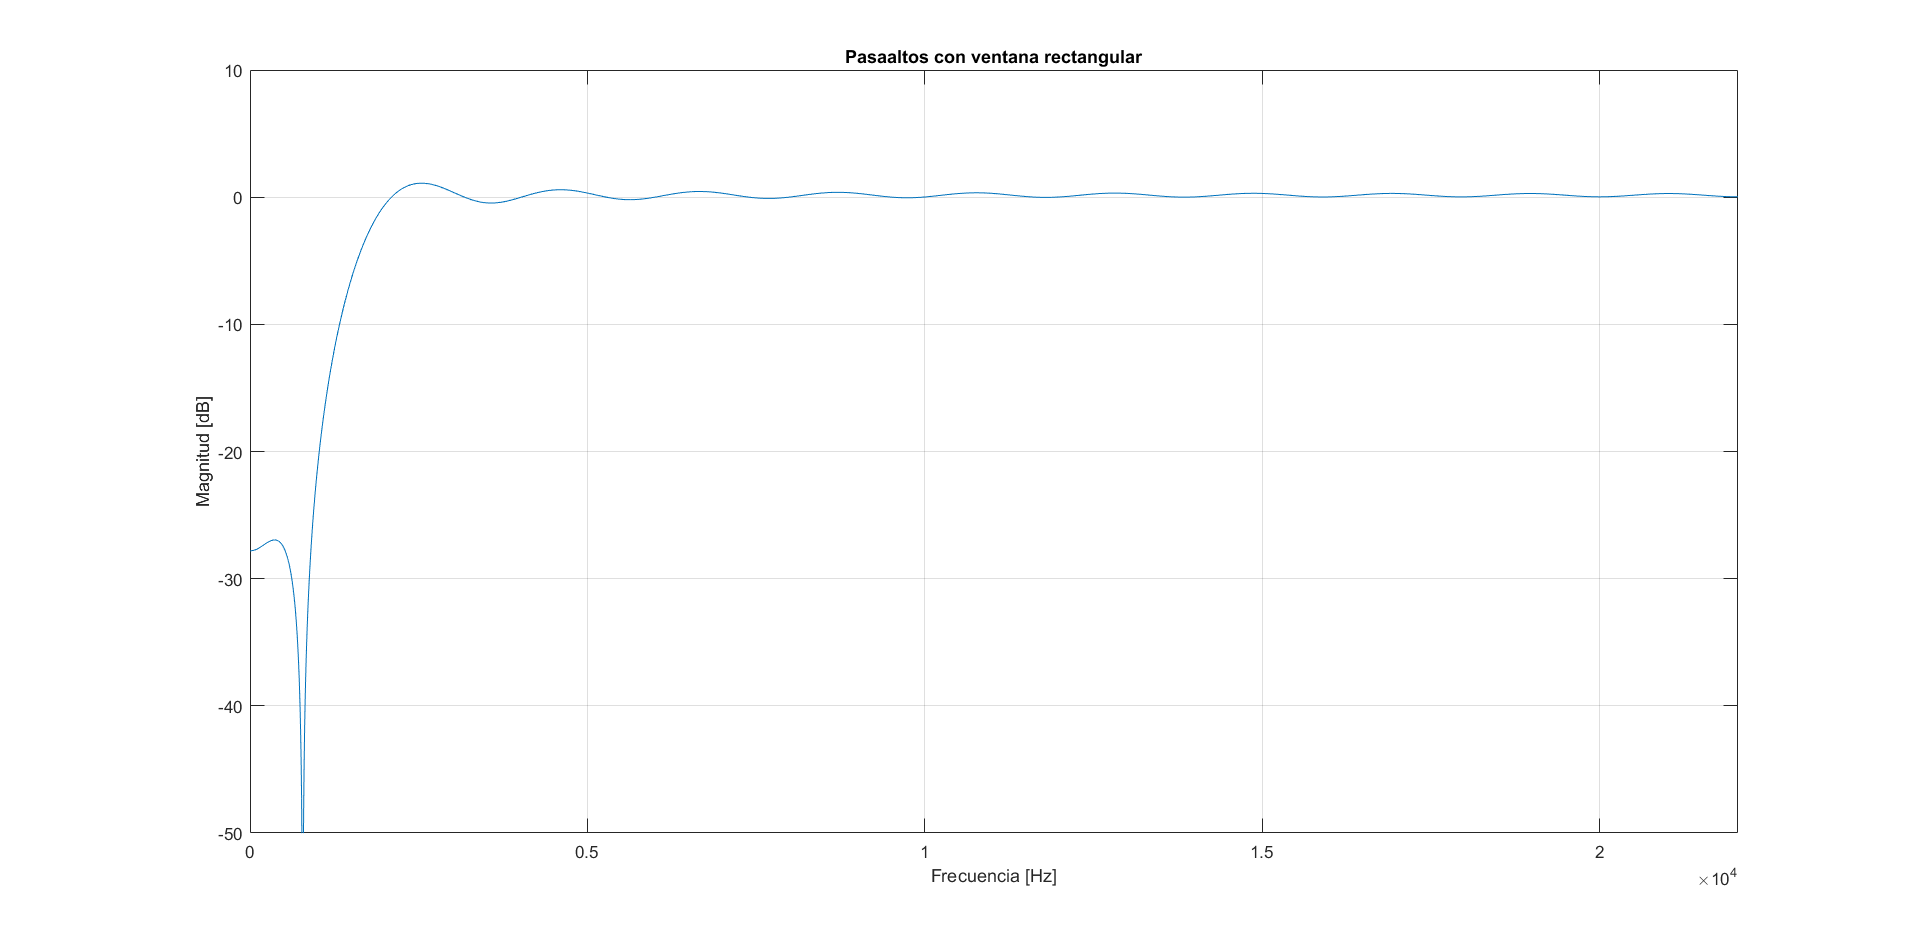
\includegraphics[scale=.35]{./images/1/recmod.png}
  \caption{Respuesta en frecuencia del pasaaltos con ventana rectangular.}
\end{figure}
\begin{figure}[H]
  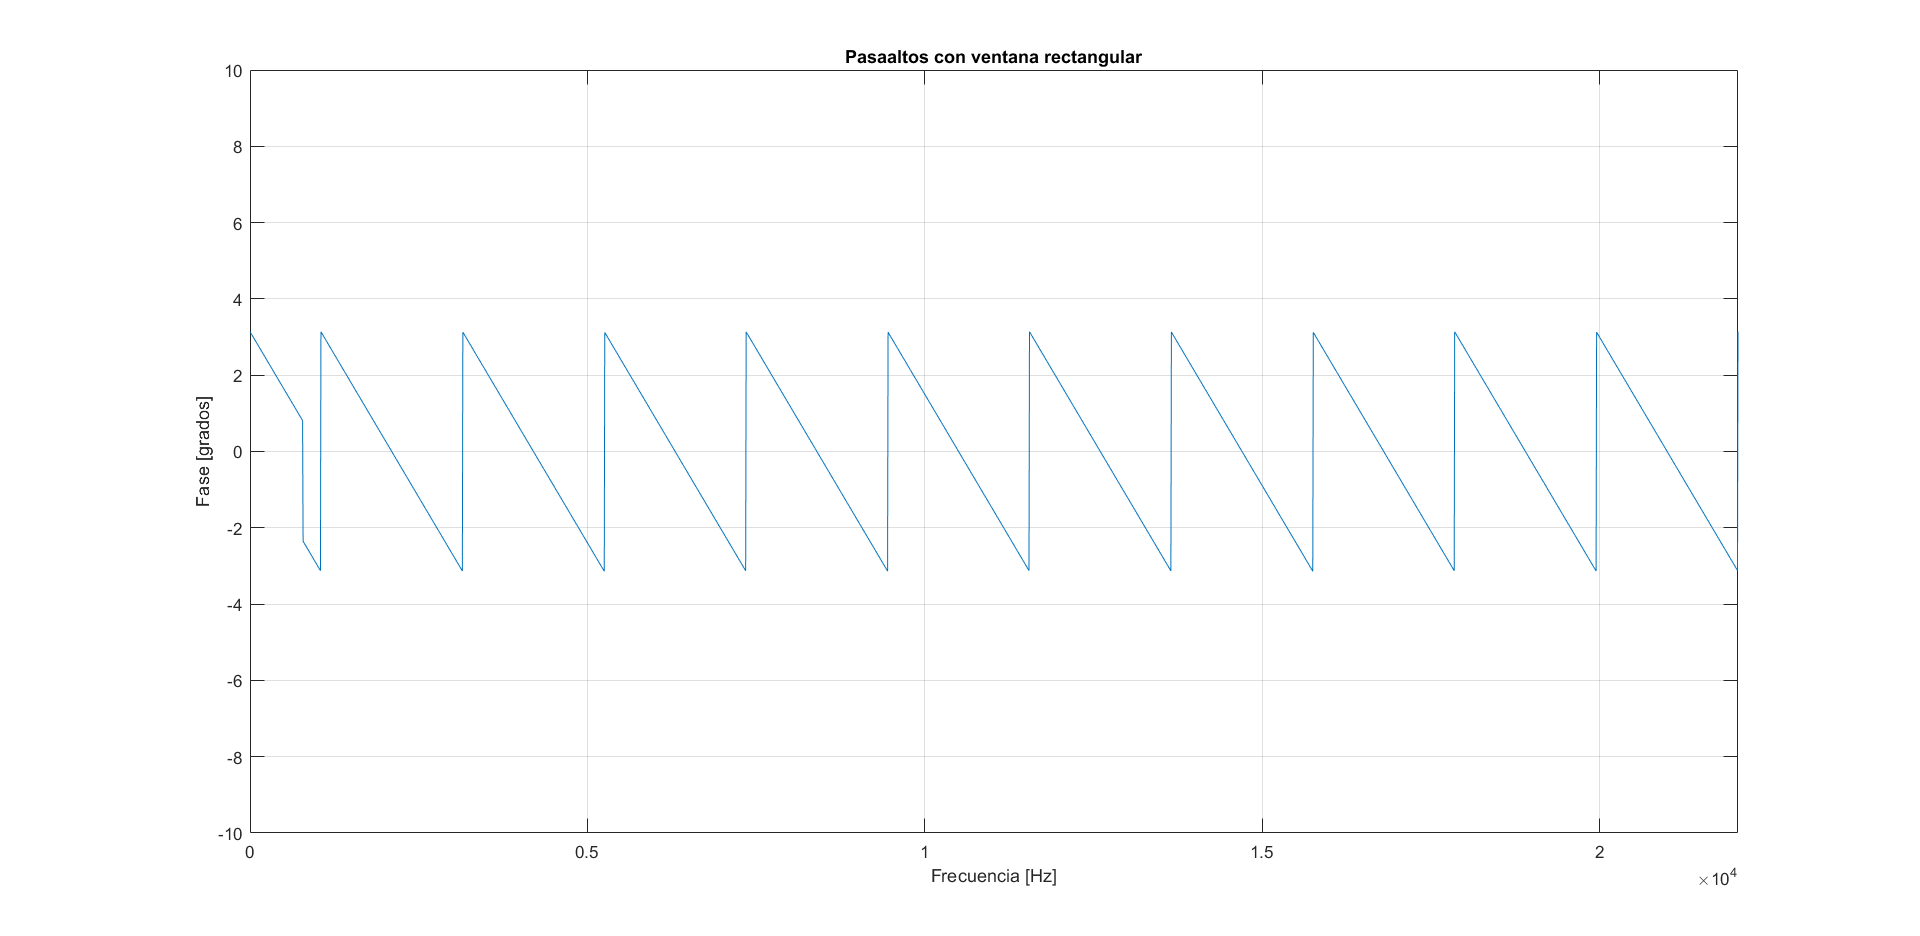
\includegraphics[scale=.35]{./images/1/recfase.png}
  \caption{Fase del pasaaltos con ventana rectangular.}
\end{figure}

\subsection{Ventana de Hamming}
La ventana de Hamming está definida por:
\begin{equation}
    \omega (n+1)=0.54+0.46\cos\left(\frac{2\pi n}{N-1} \right)  \qquad  0<n<N-1
\end{equation}
\begin{figure}[H]
  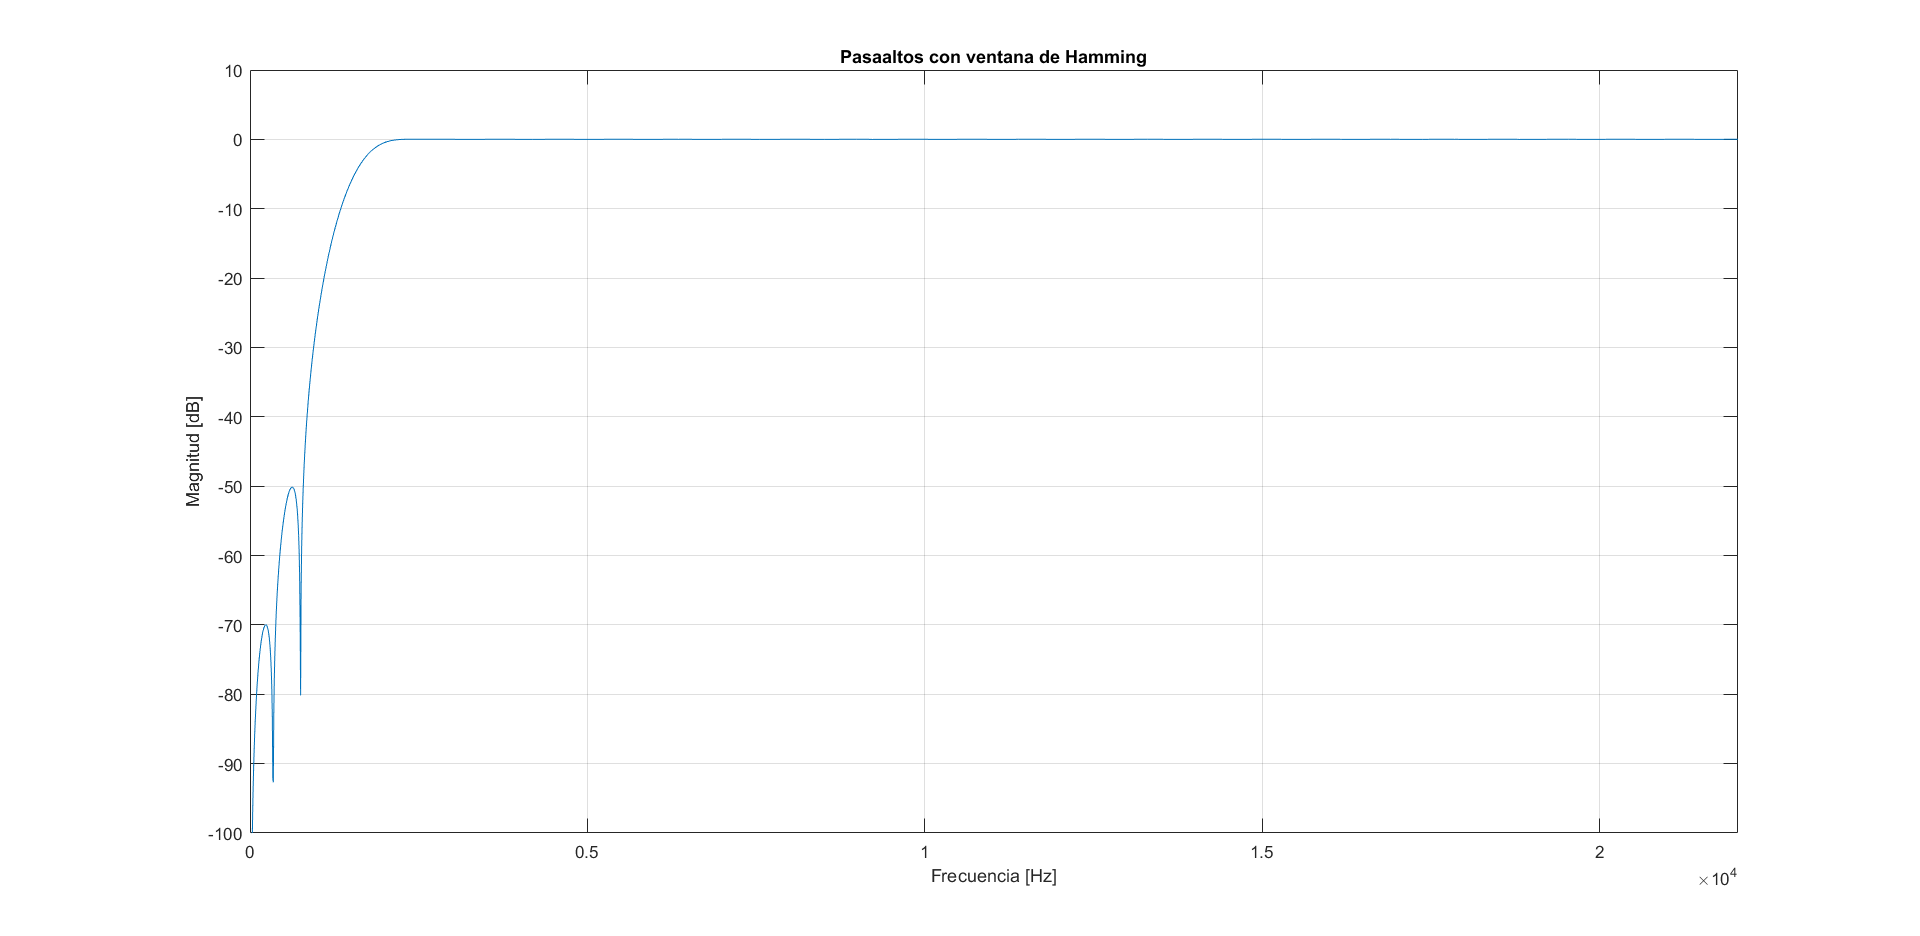
\includegraphics[scale=.35]{./images/1/hammingmod.png}
  \caption{Respuesta en frecuencia del pasaaltos con ventana de Hamming.}
\end{figure}
\begin{figure}[H]
  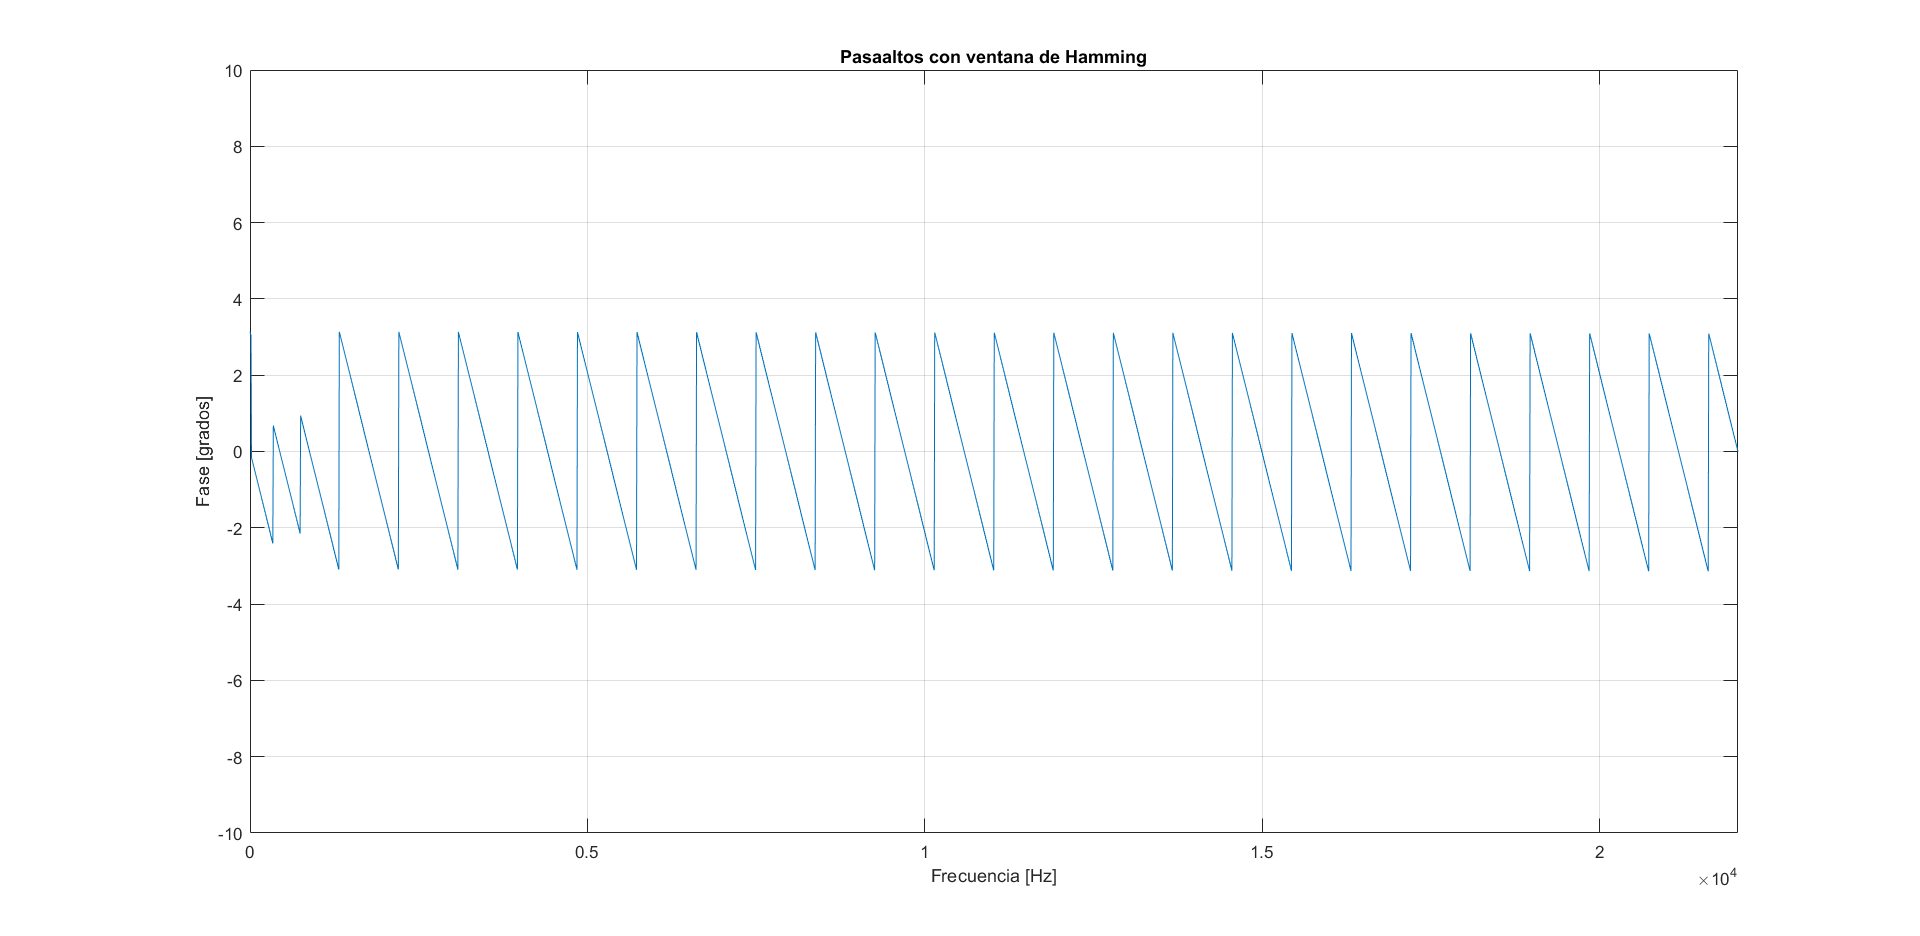
\includegraphics[scale=.35]{./images/1/hammingfase.png}
  \caption{Fase del pasaaltos con ventana de Hamming.}
\end{figure}

\subsection{Ventana de Blackman}
La ventana de Blackman está definida por:
\begin{equation}
    \omega (n+1)=0.42-0.5\cos\left(\frac{2\pi n}{N-1} \right)+0.08\cos\left(\frac{4\pi n}{N-1} \right)  \qquad  0<n<N-1
\end{equation}
\begin{figure}[H]
  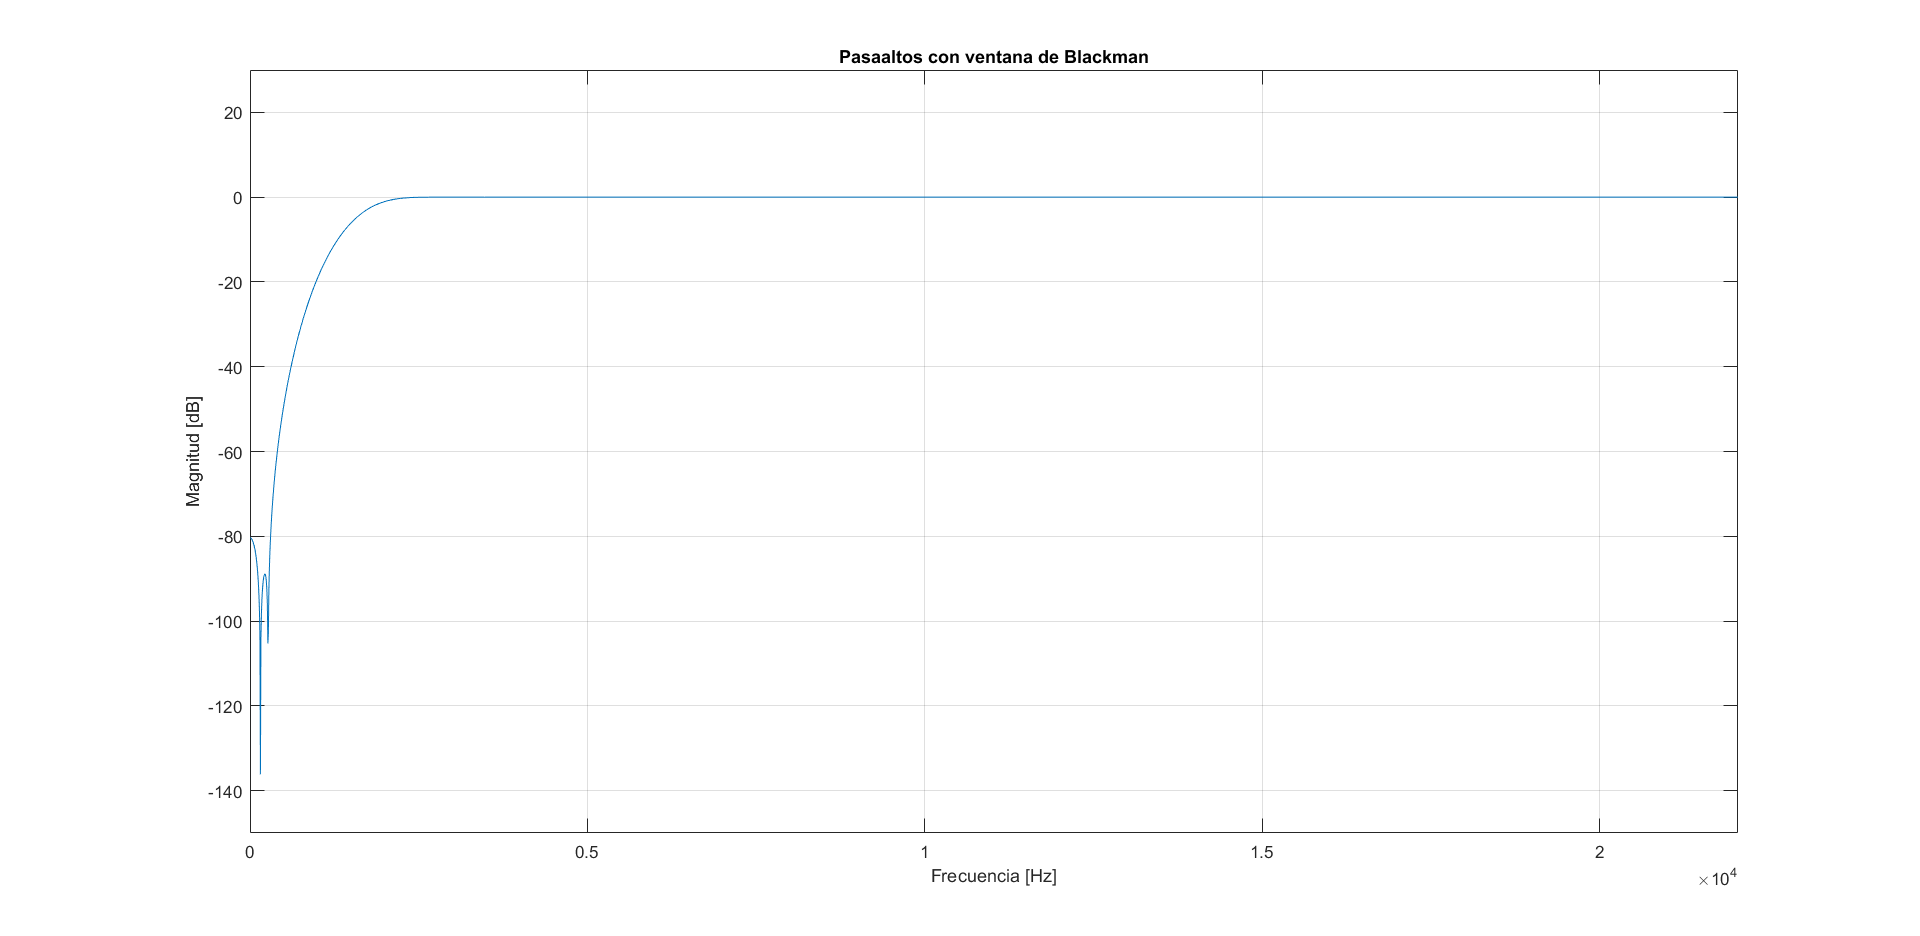
\includegraphics[scale=.35]{./images/1/blakmod.png}
  \caption{Respuesta en frecuencia del pasaaltos con ventana de Blackman.}
\end{figure}
\begin{figure}[H]
  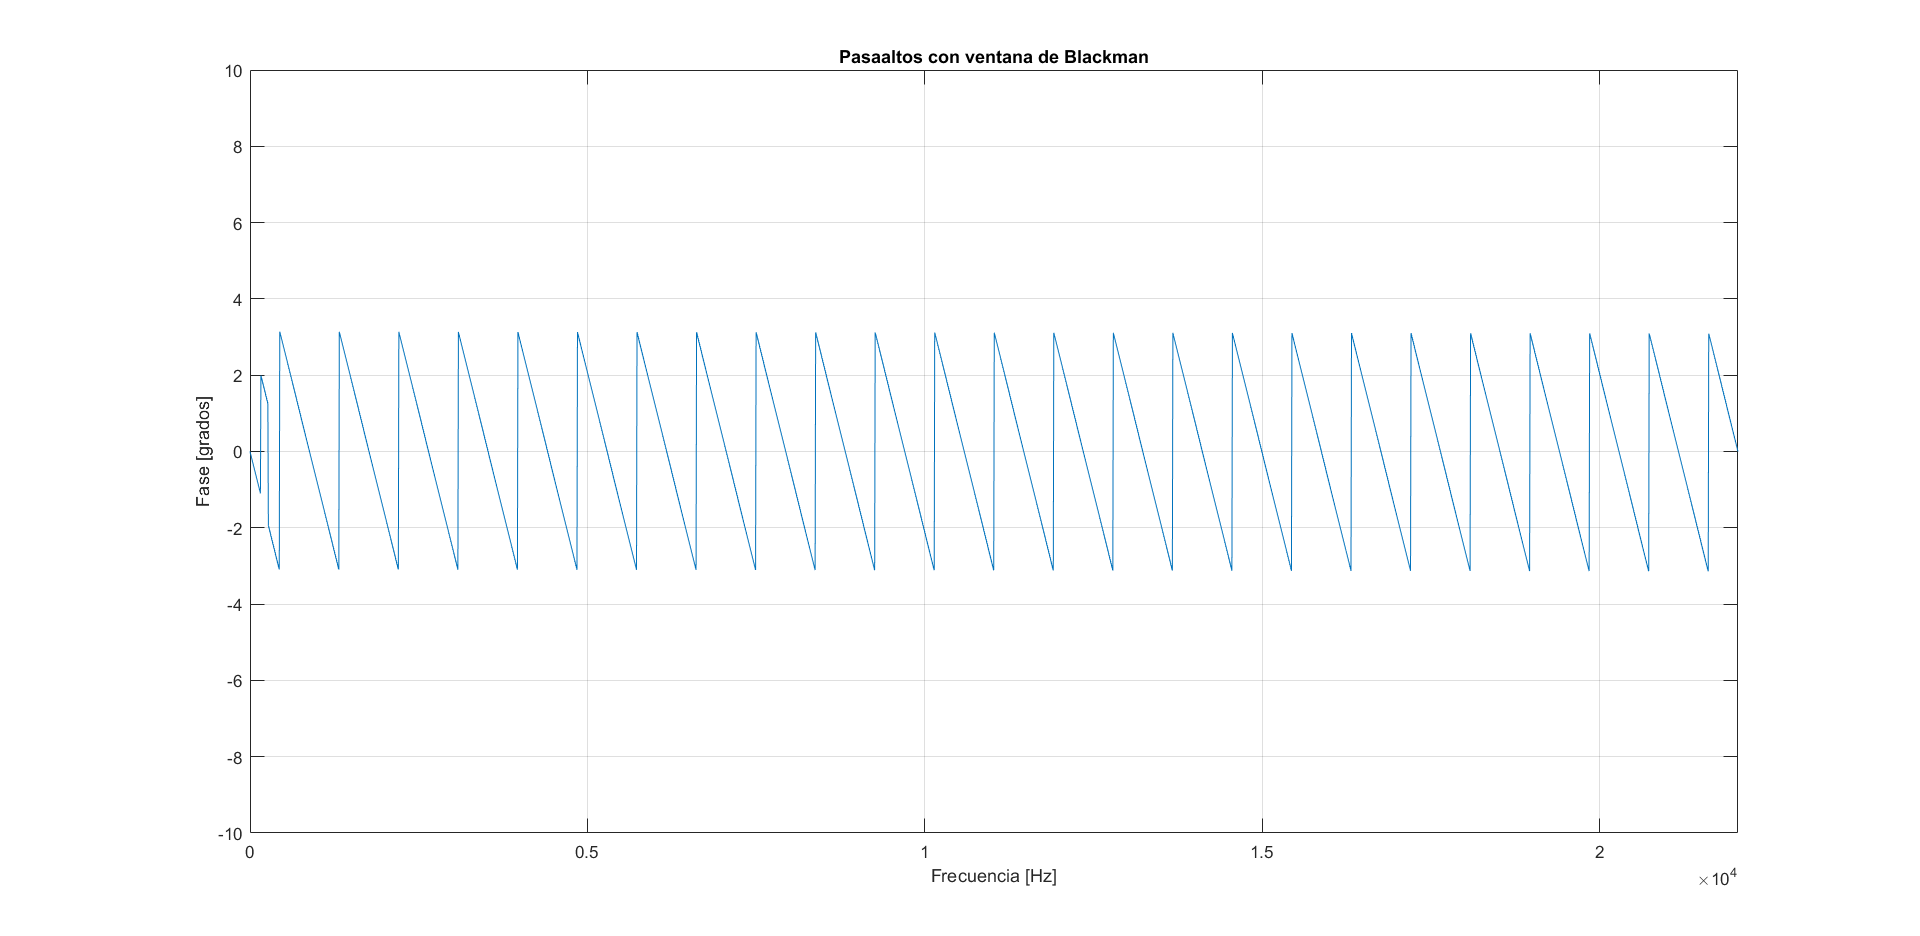
\includegraphics[scale=.35]{./images/1/blakfase.png}
  \caption{Fase del pasaaltos con ventana de Blackman.}
\end{figure}


\subsection{Ventana de Kaiser}
La ventana de Kaiser está definida por:
\begin{equation}
    \omega (n+1)=\frac{I_0 \left( \pi\alpha\sqrt{1-\left(\frac{2n}{N-1}-1 \right)^2} \right)}{I_0\left( \pi \alpha \right) }  \qquad  0<n<N-1
\end{equation}
Con $I_0$ la función de Bessel modificada de primer tipo de orden cero, $\alpha$ es un número real que determina la forma de la ventana, la relación entre el ancho del lóbulo principal y la amplitud de los laterales. El ancho del principal está dado por  $2\sqrt{1+\alpha^2}$.
\begin{figure}[H]
  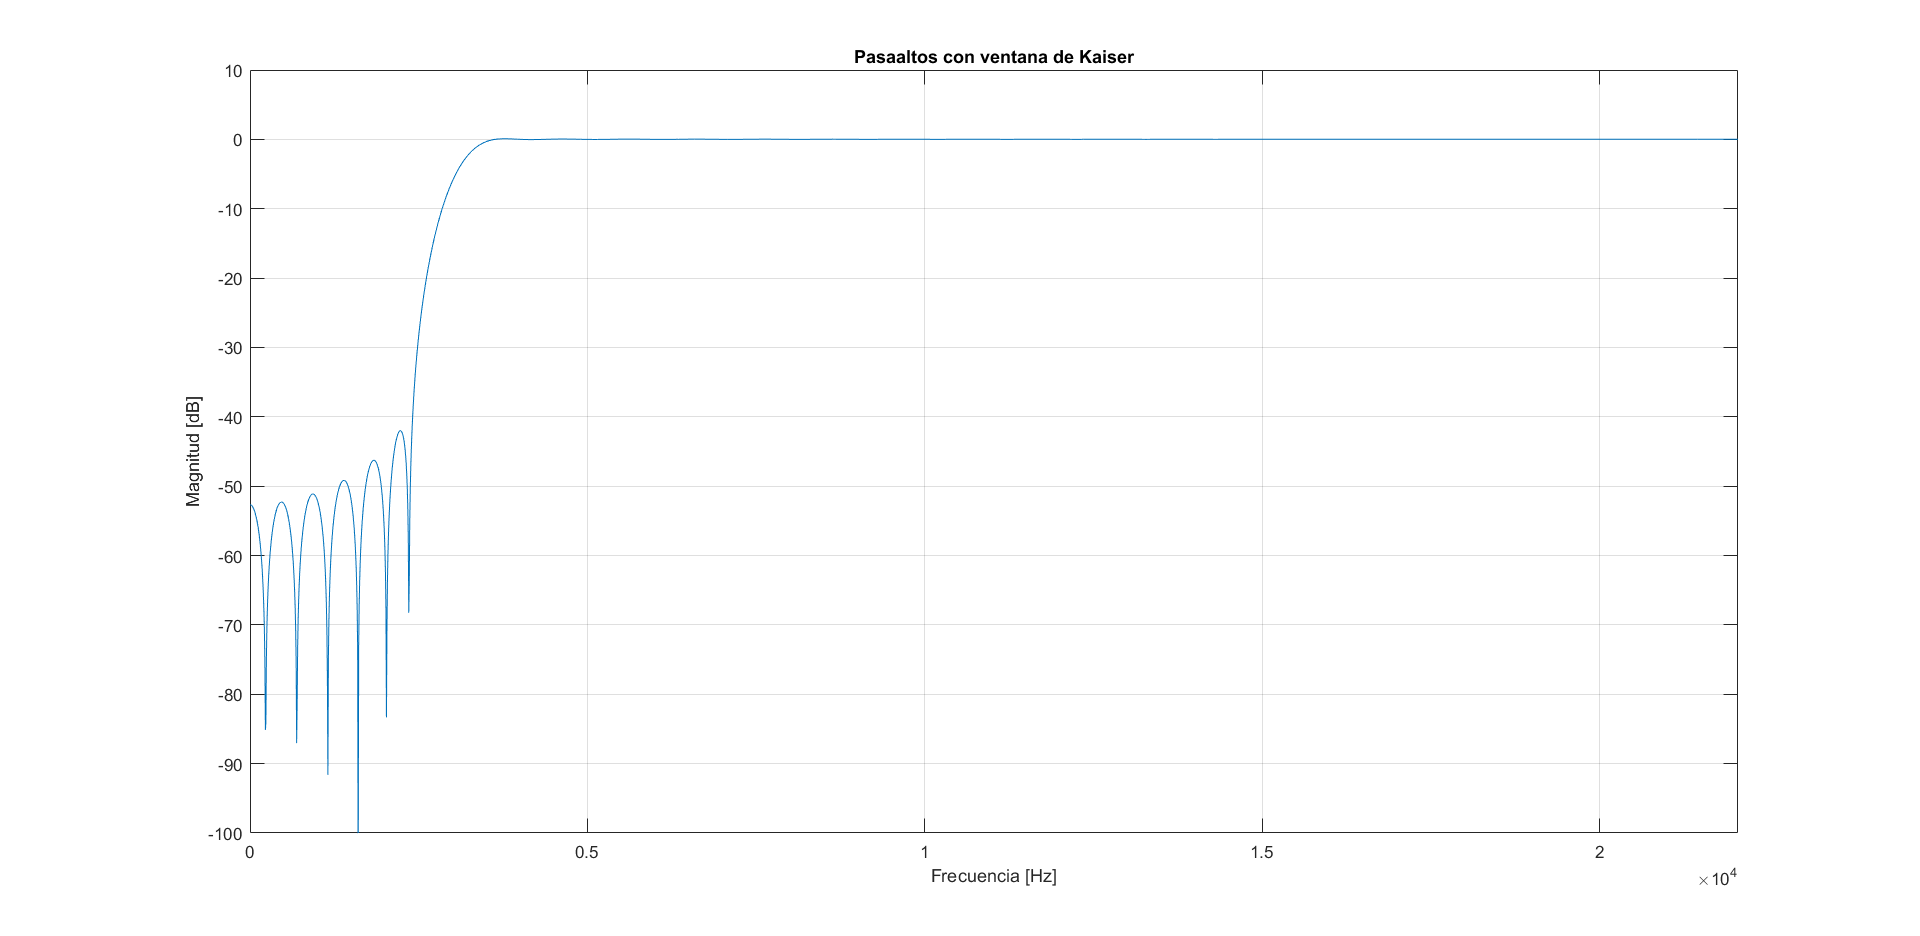
\includegraphics[scale=.35]{./images/1/kaimoduloAa40.png}
  \caption{Respuesta en frecuencia del pasaaltos con ventana de Kaiser para $Aa=40dB$.}
\end{figure}
\begin{figure}[H]
  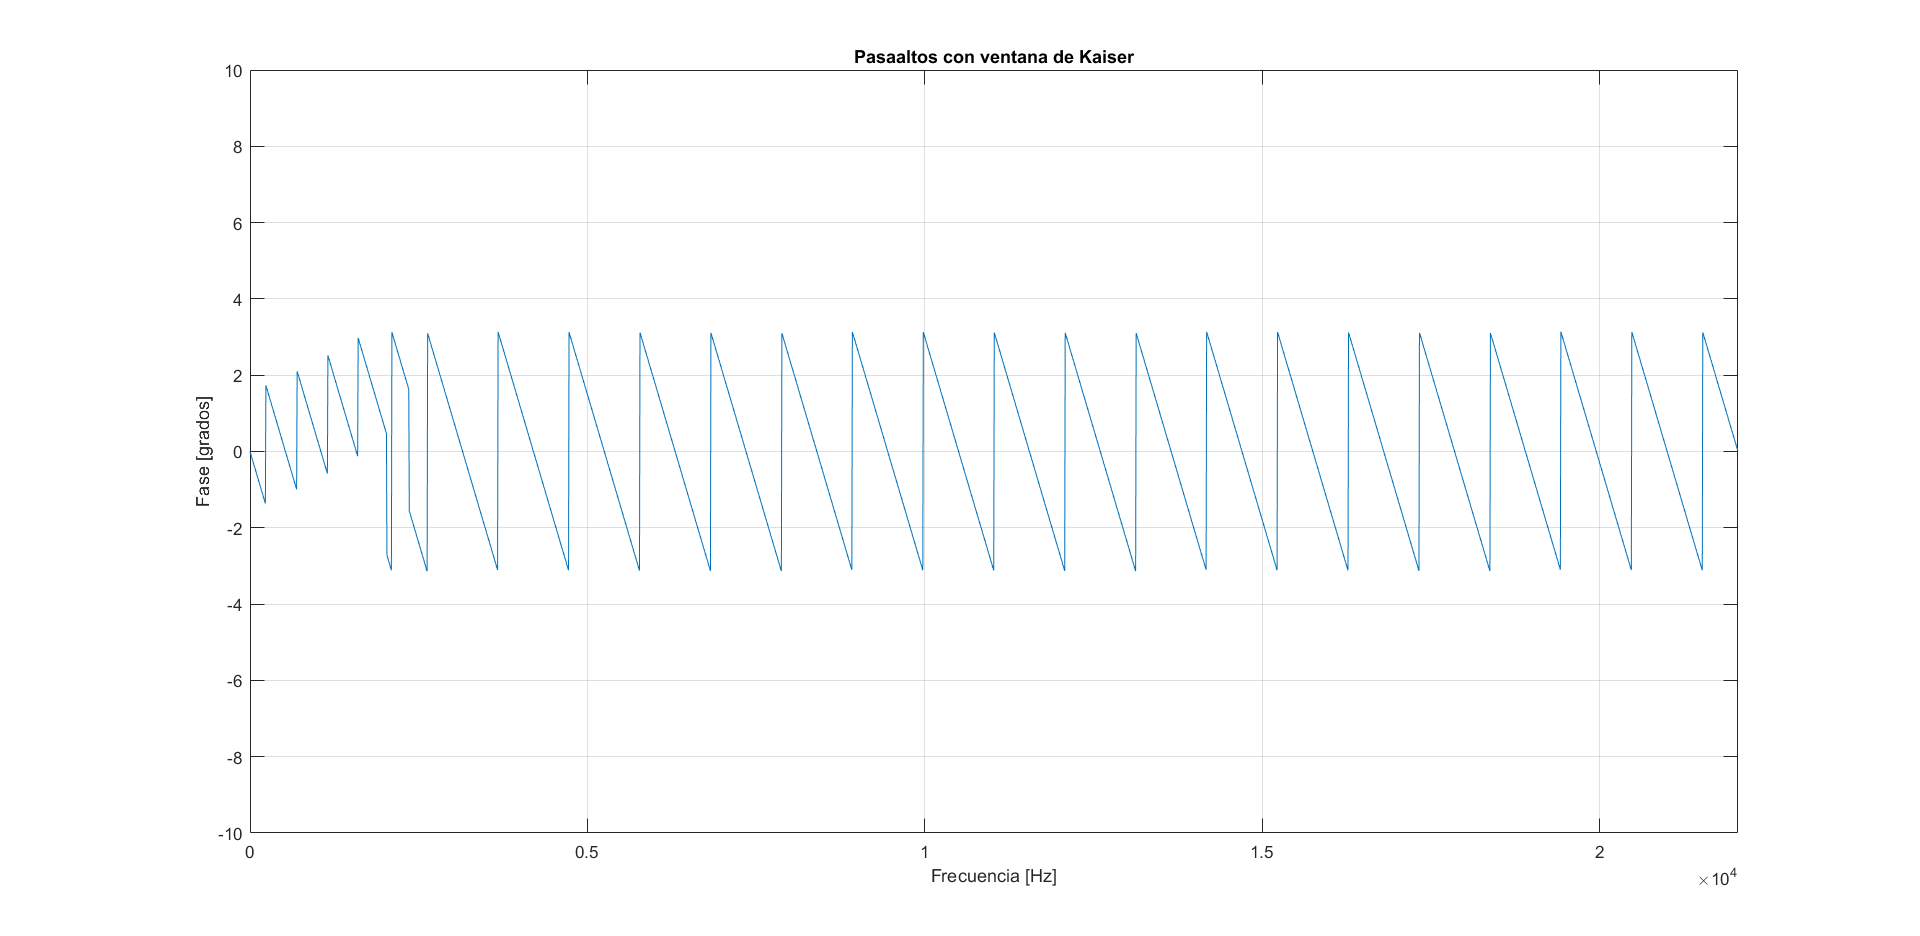
\includegraphics[scale=.35]{./images/1/kaifaseAa40.png}
  \caption{Fase del pasaaltos con ventana de Kaiser para $Aa=40dB$.}
\end{figure}
\begin{figure}[H]
  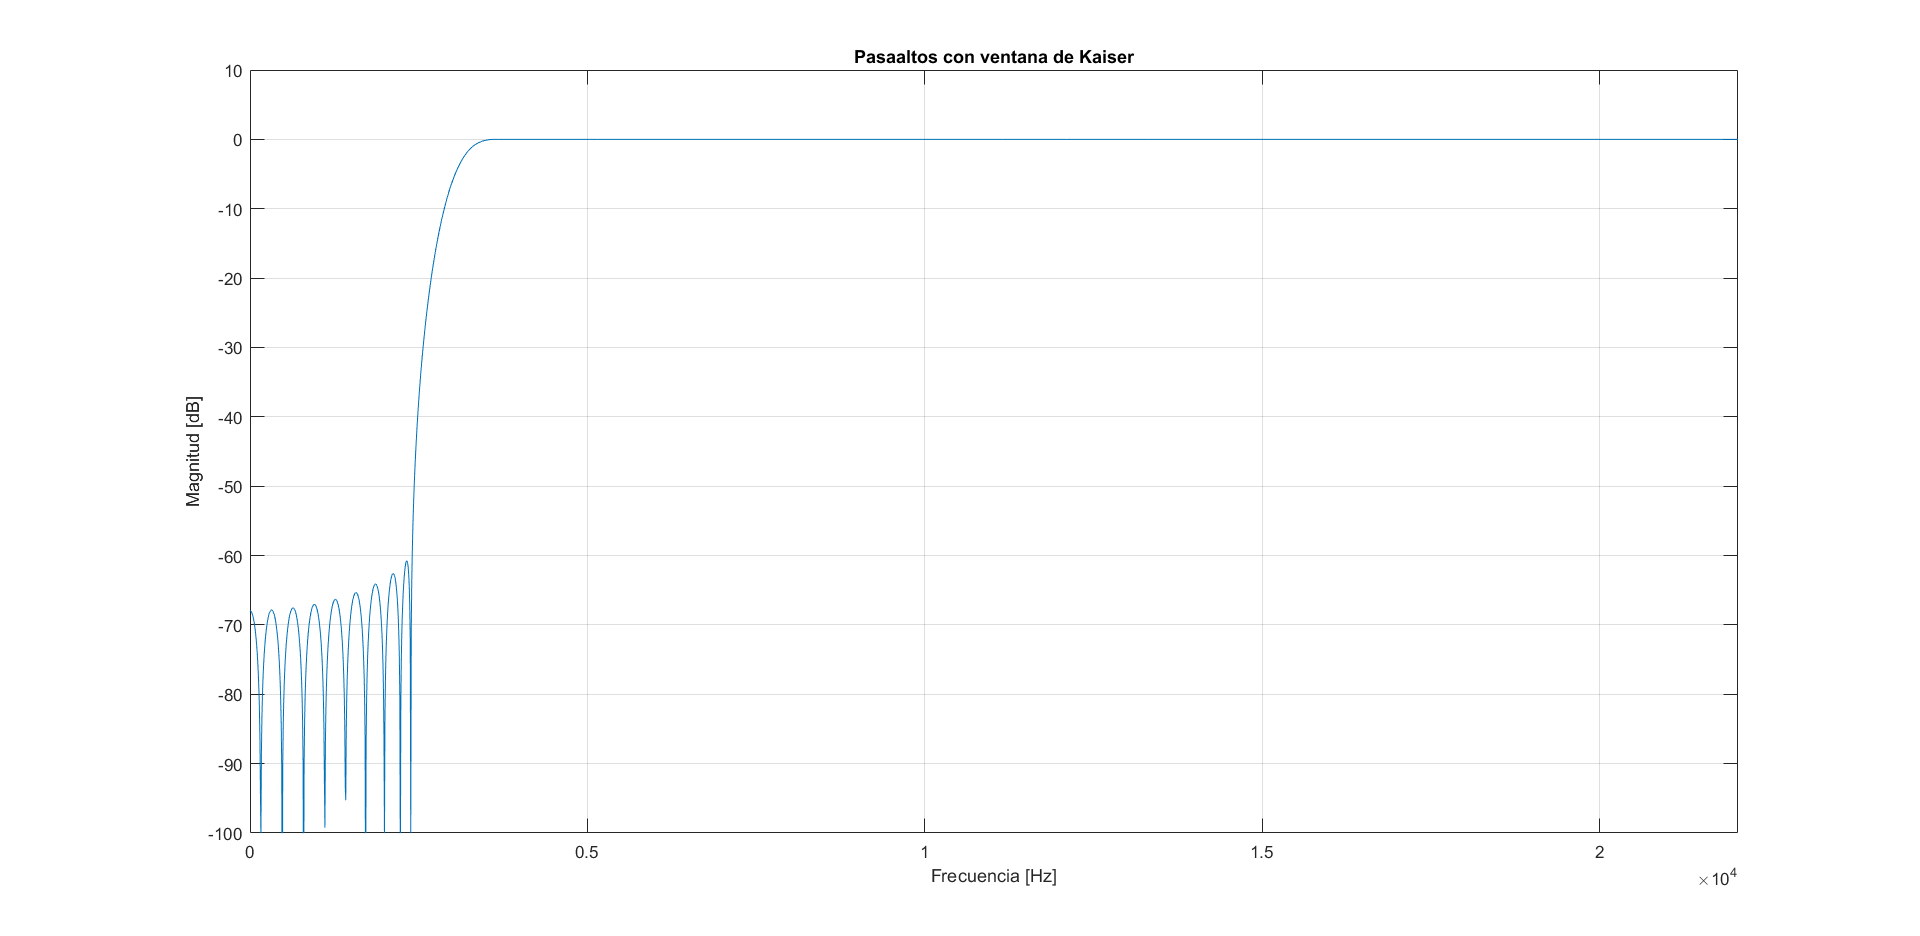
\includegraphics[scale=.35]{./images/1/kaimoduloAa60.png}
  \caption{Respuesta en frecuencia del pasaaltos con ventana de Kaiser para $Aa=60dB$.}
\end{figure}
\begin{figure}[H]
  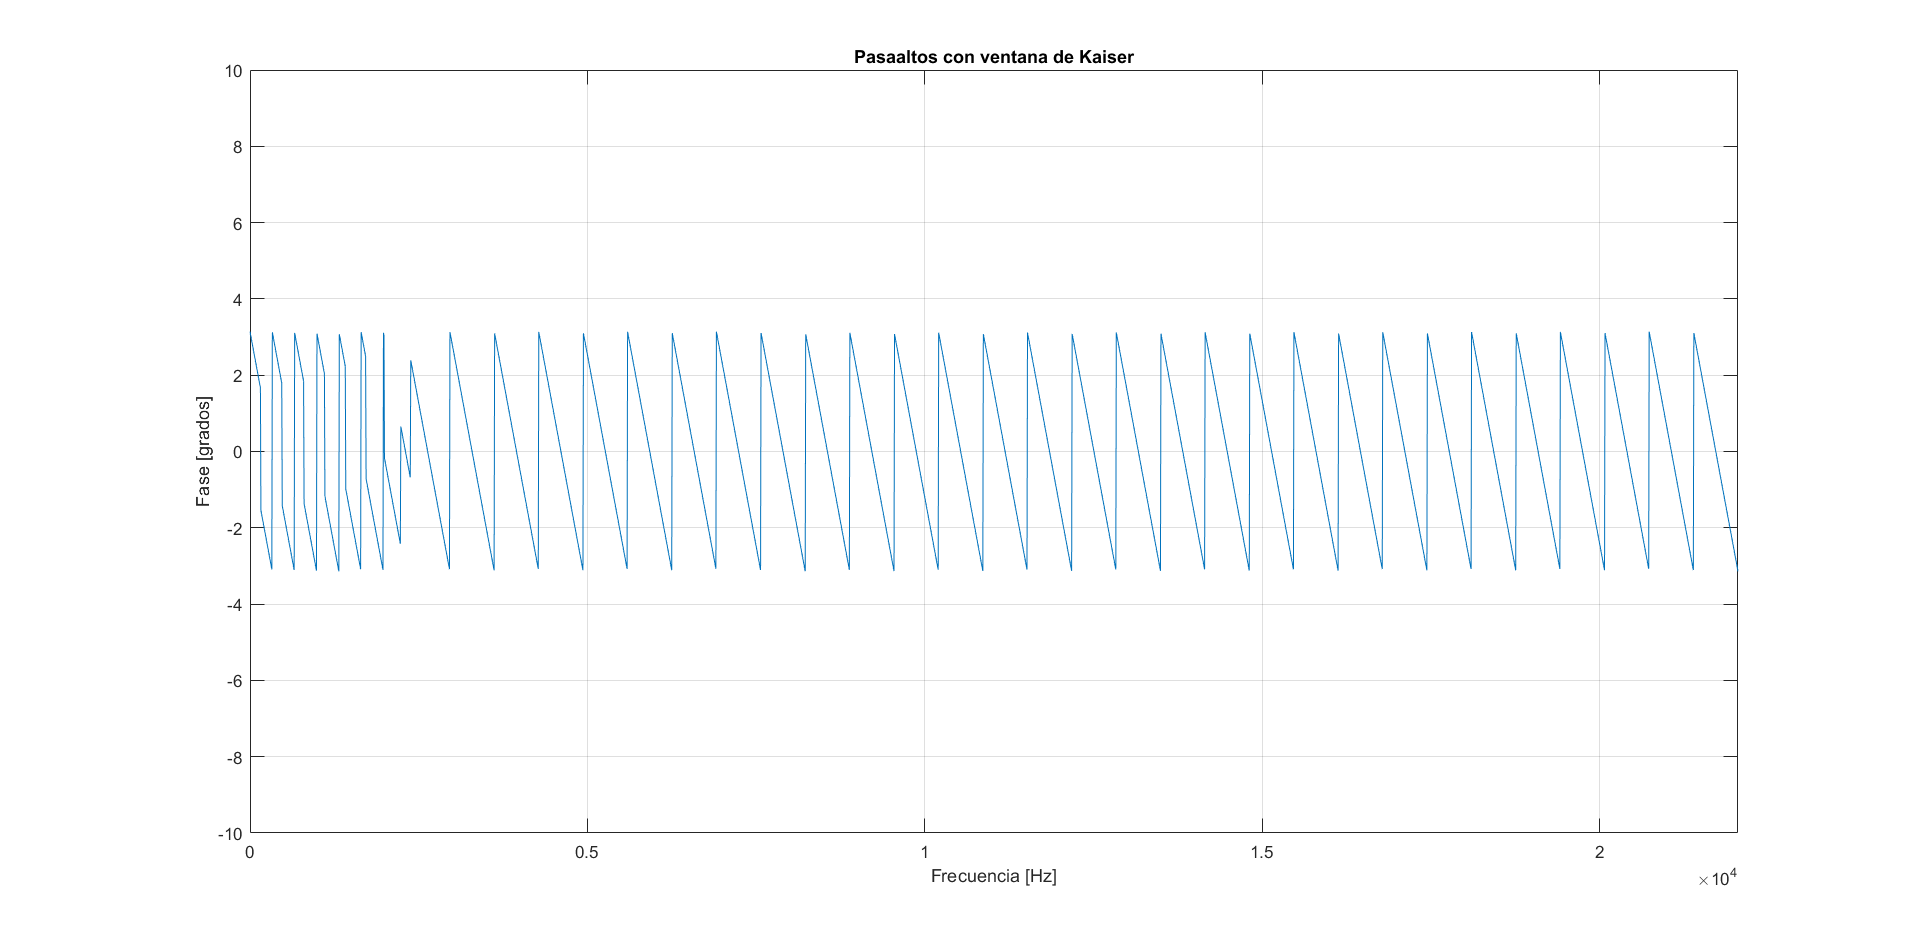
\includegraphics[scale=.35]{./images/1/kaifaseAa60.png}
  \caption{Fase del pasaaltos con ventana de Kaiser para $Aa=60dB$.}
\end{figure}


\subsection{Análisis de Resultados}

Para poder apreciar mejor los resultados se graficaron los bodes de las ventanas superpuestas, que se muestran a continuación:
\begin{figure}[H]
  \centering
  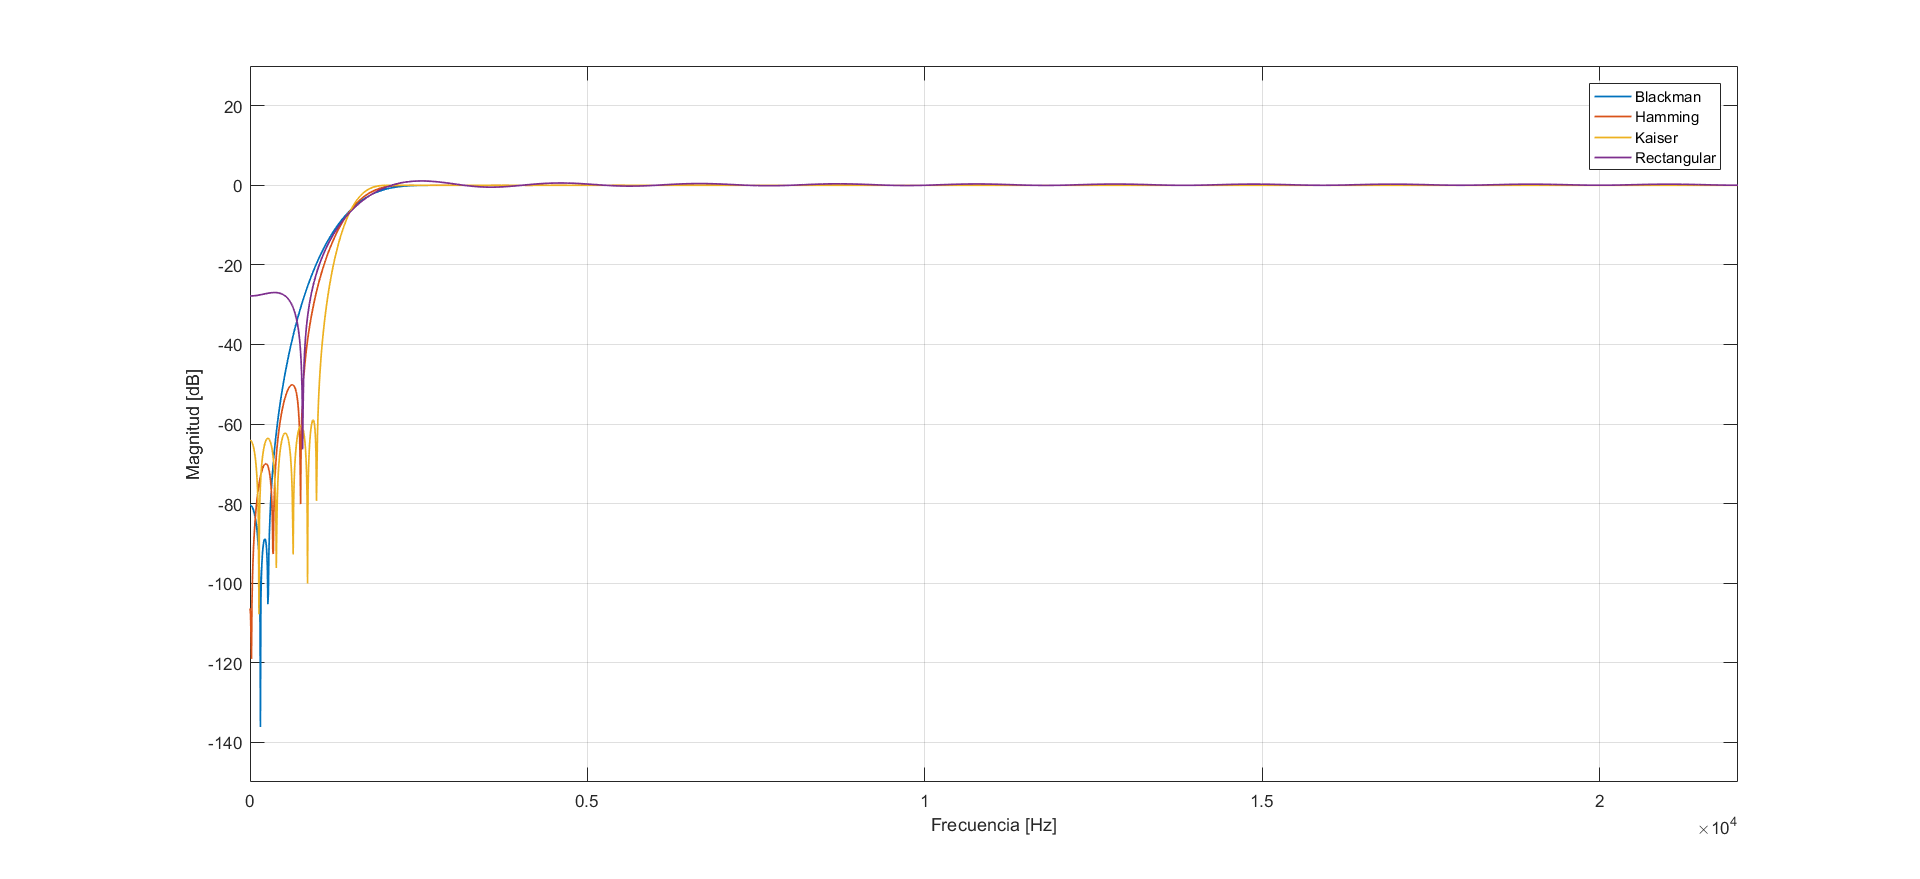
\includegraphics[scale=.35]{./images/1/modulos.png}
  \caption{Respuesta en frecuencia del pasaaltos con ventana rectangular, Hamming, Blackman y Kaiser.}
\end{figure}
\begin{figure}[H]
  \centering
  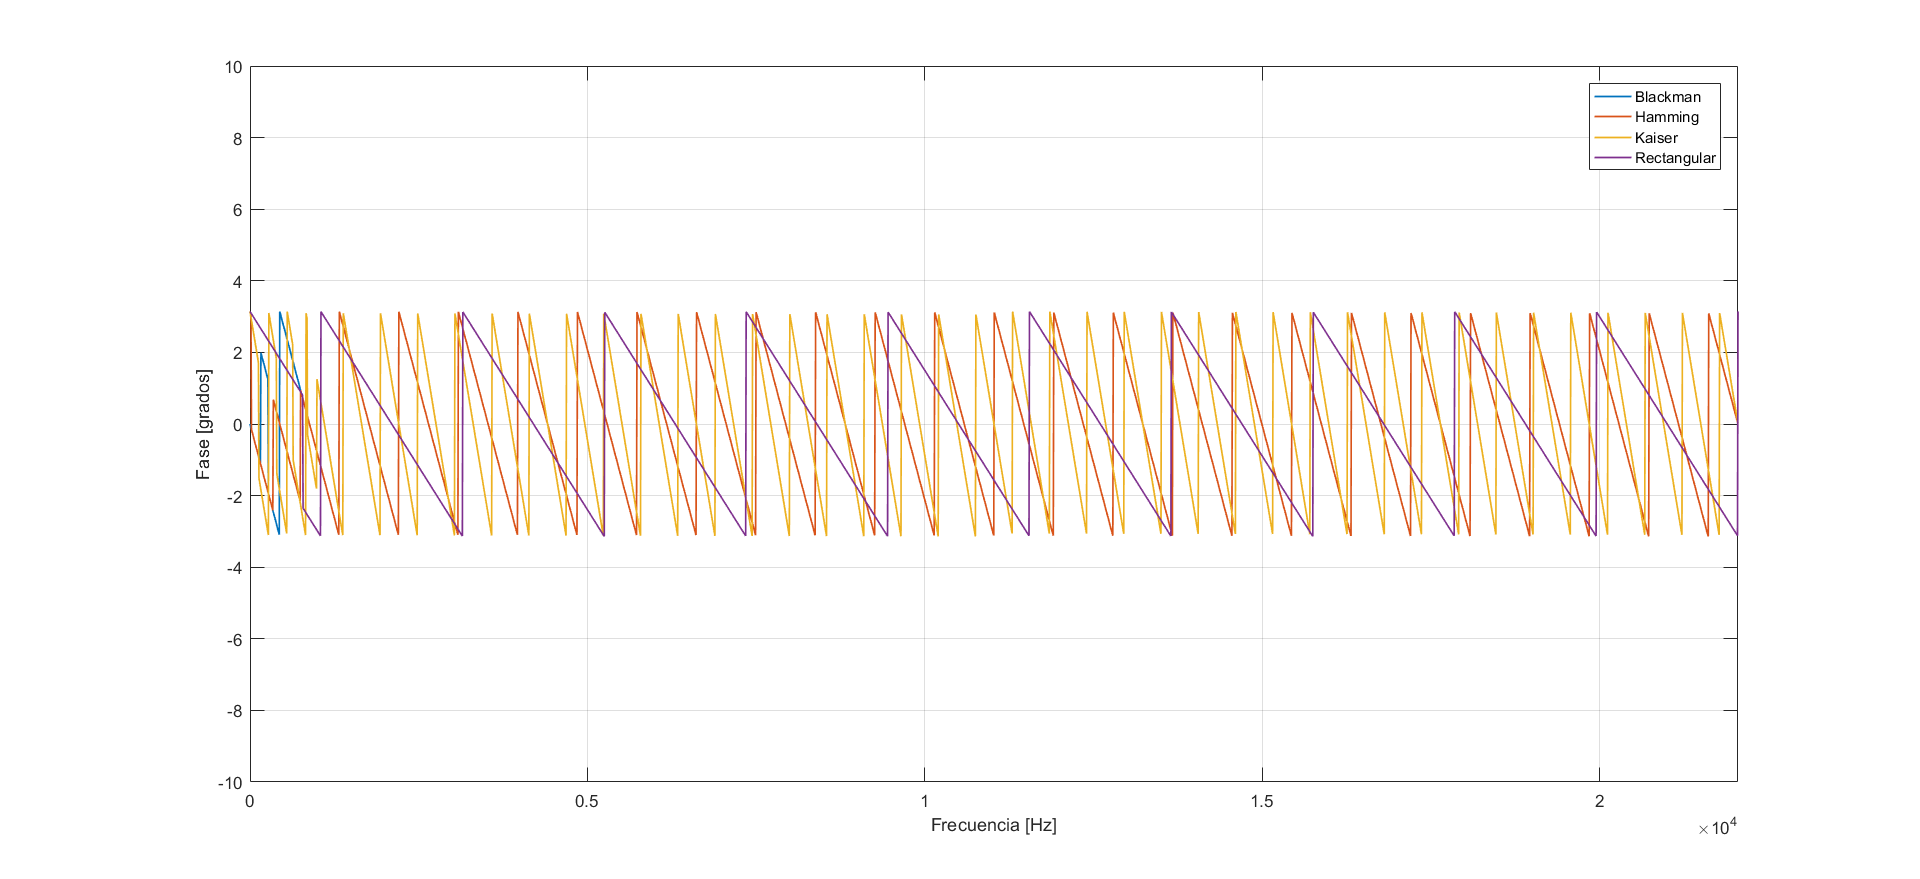
\includegraphics[scale=.35]{./images/1/fases.png}
  \caption{Fase del pasaaltos con ventana rectangular, Hamming, Blackman y Kaiser.}
\end{figure}

En principio se puede observar que se consigue una mayor atenuación en los lóbulos laterales con la ventana de Blackman ($80dB$), frente a las otras ventanas propuestas. En particular, con la ventana rectangular es donde se consigue la menor atenuación. Por otro lado, la ventana de Kaiser permite obtener el $N$ óptimo para el caso, aprovechando el parámetro $\alpha$ que permite variar, en forma continua, el ripple desde los valores de la ventana rectangular, hasta los de Blackman. A mayor $\alpha$, mayor $Aa$, y mayor el ancho de la banda de transición. Una vez elegido el $\alpha$ que satisfaga las atenuaciones deseadas, se ajusta el $N$ para satisfacer el ancho de la banda de transición pedido.
\par En cuanto a las fases planteadas, la rectangular es la que tiene menor ancho del lóbulo central, por lo que los ceros de transmisión aparecen primero en ella. La de Blackman es la de menor selectividad y mayor ancho de lóbulo central, sucediendo a la inversa que la rectangular. En cada  una de ellas, luego de cada cero hay un cambio de signo (salto en $\pi$).
